\chapter{Application}
\section{Data Explanation}
\label{sec:data}
\begin{comment}
We have now laid down the theory of what we want to do describing all of the choices we may need to make, so now we will put it in action. The data that we will apply it to is a dataset from M.D Anderson Cancer Center. The data is a collection of about 1500 patients at MD Anderson who have breast cancer that has metastasized to the brain, about 100 clinically relevant covariates, along with their survival status and time.
\end{comment}
Unfortunately, as of October 23rd, we are still waiting for final approval from the PI of the project and the IRB. I want to get the proposal out to y'all though. So, what I will do in this section is describe what I will do, and once I get approval, I will fill in the tables and plots. In the meantime, I will put in <whatever> where something that uses the data should be. The IRB protocol is RCR03-0931, but neither Dr. Hess nor myself are on the protocol, because it is out of date. We are in the process of getting it updated, and plan to have it done by the time I defend this thesis

Now that the theory is in place, we can apply it to some real data. The dataset that I chose to analyze is a dataset from MD Anderson Cancer Center, with permission from Dr. Bugano, Dr. Ibrahim, Dr. Hess and <whoever else needs to be thanked>. This dataset has historical records of 1514 MD Anderson patients who have had breast cancer that has metastasized to the brain. There are lots of covariates recorded (about 90, most with some missingness), a few different treatments, as well as survival endpoints (which are all observed). The data can be broken down into a few parts; subject data (like age range and race), cancer type data (like stage, type, status), pre metastases data (like treatment types), clinical observations (like headaches or nausea) post metastases data (like treatment, type of brain metastasis), and survival (survival of different events and censoring indicators). In figure \ref{fig:missingplot} we see a plot of the missingness in the data. This data is exemplary for this task because it is large, survival amenable, has missingness and is a prime candidate for imputation, and has treatment variables that are not given in an RCT.
\begin{figure}[h!]
  \centering
    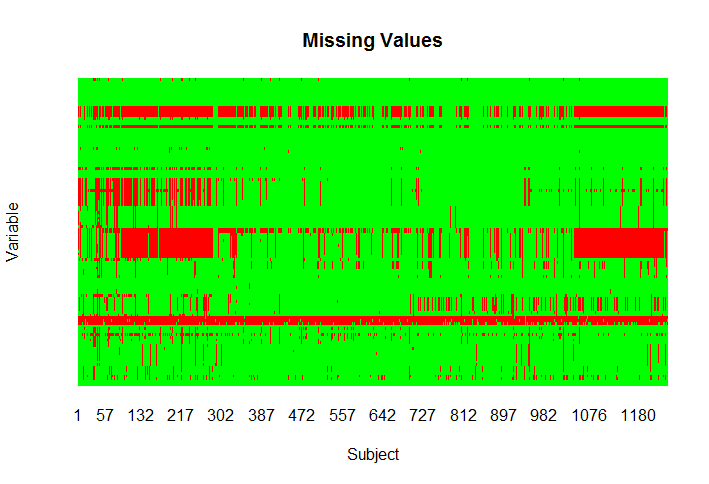
\includegraphics[width=0.8\textwidth]{missingvalues_plot.png}
  \caption{Visualization of missingness in the cancer dataset}
\label{fig:missingplot}
\medskip
\small
Along the horizontal axis is the subject, and the vertical axis is the covariates. \textcolor{green}{Green} denotes observed values whereas \textcolor{red}{red} is missing. The covariates with the highest missingness are three genetic measures, as well as some clinical assessments.
\end{figure}

Our first step is to clearly define what we would like to find. There are many interesting questions we could ask and answer from this data because of the amount of data available, but the question I will focus on here is survival in two different settings. In the first, we will explore the treatment effect of Capecitabine (a chemotherapeutic agent) versus other chemotherapeutic agents versus no treatment. In the second, we will look at the effect of two HER2 directed drugs (Lapatinib versus Trastuzumab) versus no HER2 targeted drugs in a subset of the patients who are HER2+
It isn't vital to understand what these drugs do, but the interested reader may want to look at appendix \ref{app:apdxb} for a very basic overview of breast cancer and the methods of how different drugs work. For a much more detailed analysis and other clinically relevant questions, see !!Hess, Bugano, Berliner!! This is the project that this research was forked off of, although it will probably not be published by the time this thesis is. 
\section{Imputation}
We first need to impute the missing data. This is a challenging task, because of the attention and care that needs to be given to imputing about 90 covariates with missing data. But we need these covariates to be imputed properly because; they have the potential to be useful as predictors for other covariates, they might be something we are actually analyzing (now or later), we have spent the money to collect the data, and it strengthens the MAR assumption. As well, it is my opinion (and probably a consensus among applied statisticians) that is better to have too many covariates than not enough. After all, variable selection can be performed if there are too many covariates. 

Our data is quite high dimensional, and there are a many binary variables as well as a handful of strictly positive covariates, thus JM imputation seems inappropriate. Instead, FCS models seem better suited. We will be using the R package mice \cite{VanBuuren2011} because it is easy to use yet powerful. 

The model is set up by hand, following the advice from \cite{VanBuuren2011}. It took about three weeks to set up and check. This was because the number of covariates was huge, and checking the imputations after a change was time consuming. It would not take this long for a smaller dataset. Creating valid imputations is a skill that lies somewhere between an art and a science, so it takes the theory to know what to do, and trial and error to see if you've done it correctly.

The first task we need to do is to assess the missing data mechanism. As we have discussed before, there is no test to determine what the mechanism is. It is very unlikely that the data is MCAR (which we typically associate with random/accidental deletion), so it is between MAR and MNAR. We have so many different covariates, and it could reasonably be assumed that the missing data we have could be explained by the type of disease, its stage, the subject's age, their standardized assessment, and their survival time, among other things which we have collected. So it would be reasonable to assume that the missing data mechanism is MAR, and thus imputation can be confidently used

For each covariate with missingness, we need to decide the form of the imputation model that will be used for imputation, and what predictors will be used in it. Most of the covariates that needed imputation were either binary or categorical, so the most popular model chosen were logistic regression and predictive mean matching. The continuous variables were often selected via regression or predictive mean matching. I decided to be very forgiving, and use nearly every reasonable predictor for each missing covariate. I did this to bolster the MAR claim, and avoid variable selection. Van Buuren proposes measures called influx and outflux to determine how worthy and connected each covariate will be as a predictor \cite{VanBuuren2012}. An ideal variable to use as a predictor would be one with an influx and outflux near one. I used all predictors except those that had very poor influx and outflux. Unsurprisingly, these were the ones with extreme missingness<influx and outflux plot>

Once the choices had been made, I needed to run the imputations by trial and error. This took a considerable amount of time, because after every change made, I had to rerun the imputation and reassess convergence and validity of the imputation. I did trial and error for model and predictor specification until the data seemed like it could have reasonably been observed.

For the final imputation, I decided to impute $m=50$ datasets and 40 iterations for each. Mice generally converges quickly (within 5 or 10 iterations), but by setting the number of iterations so high, it is as if we are setting a burn in period, and then taking our sample. The number of datasets was selected to be 50 because in general, according to Reiter the number of datasets should be more than the imputations \cite{Reiter2008}, and while there is no consensus about how many imputations to do, the modern research argues that the more the better. Research by White et. al  says that you should choose $m$ to be about 100 times the percentage of incomplete cases (for the analysis at hand) \cite{White2011a}. The data used in our analysis has about 30\% missingness, so coupled with Reiter's advice, I chose to impute 50 datasets.

After the final model for each covariate with missingness has been set up, we need to run it and save the results. For 50 datasets, 40 iterations, the algorithm runs in about 4 hours, and for 50 datasets with 100 iterations, it took 11.5 hours on a computer with 4 GB of ram and 4 cores .While this seems like a long time, this process only needs to be done once and requires no human interaction, so it can be run overnight and then never need to be touched again. I ran it for 100 iterations to see how the run time scaled, as well as to check how the chains behaved and to see how the analyses differed. The results between 50 and 100 imputations were very similar. As well, there is hardly any confidence gained going from 50 to 100, and having such large objects in memory can be harder to work with.

We need to check our final imputations for convergence and reliability. Convergence is assessed by looking at plots of covariate mean and standard deviation by iteration, as can be seen in figure \ref{fig:traceplot} There are 80 plots to check, so I cannot show all of them in this paper, I only show some interesting ones. According to van Buuren ``the different streams should be freely intermingled with each other, without showing any definite trends. Convergence is diagnosed when the variance between different sequences is no larger than the variance with each individual sequence'' \cite{VanBuuren2011}. Looking at these plots, this certainly seems to be the case. Other authors suggest using a more formal statistical tests such as $\hat{R}$< rhat> to assess convergence by looking at the within versus the between variance, so I also display that (values near 1.00 are ok and values greater than 1.1 indicate that the chain should be run for longer). Diagnostic plots are viewed to ensure that the imputed data is similar enough to the real data.< A few of the plots have been replicated here>. To see all of the plots, go to the shiny app/ R package (do this if enough time, also see about security. (Might just need to make it be �available upon request�). As we can see, not all of the imputed data follows the distribution of the observed data exactly, but for the majority of the plots, the data look like they could have been real data.

\begin{figure}[h!]
  \centering
    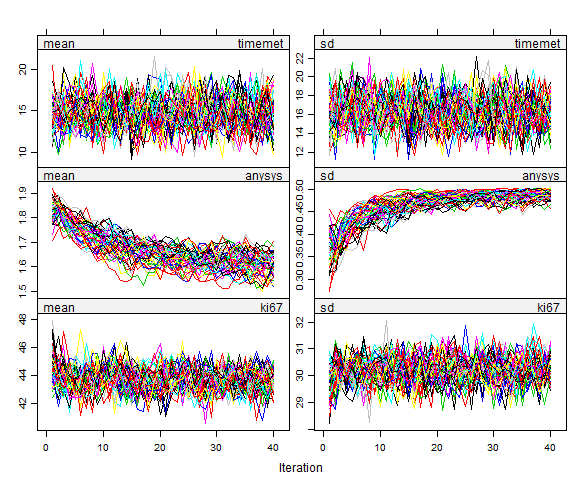
\includegraphics[width=0.8\textwidth]{traceplots.png}
  \caption{Selected plots of imputation mean and standard deviation by iteration}
\label{fig:traceplot}
the highest missingness are three genetic measures, as well as some clinical assessments.
\end{figure}

\section{Survival Analysis}

Now that the datasets are imputed, we are ready to run our models on them.  Before we begin though, we should check the models on the available cases, to make sure that the model assumptions are met, and to get an idea of how the importance of each part of the model. The available case models were run and the assumptions were checked, and all of them passed. You can see the results, alongside the MI values throughout this section.


It should be noted that in all of our survival analyses, we will be doing a landmark analysis. Landmark analysis means that we don't start the analysis at time 0, rather, we start it at a different time later than 0. In Dr. Hess's words, ``Since the brain metastases treatment data was necessarily determined after the diagnosis of the brain met, it is not appropriate to use this data as baseline covariates in the analyses. Only covariates known at the time of diagnosis can be used in this fashion� we can do a landmark analysis by estimating when the vast majority of patients would had their brain met treatment choices started and starting our analyses at this point ''. After speaking with subject matter experts (Dr. Bugano and Dr. Ibrahim), this landmark time was determined to be 2 months. 

The first result that we will check is the Kaplan-Meier curves for the imputed data. The available case analysis shows that Lapatinib and Trastuzumab are quite close to each other, while having no HER2  directed treatment being much lower. For the chemotherapeutic drugs, available case was X,Y,Z. The log rank test statistic is X, with pvalue Y, indicating Z ,and these results can be seen on <table whatever>. The pooled KM estimate was found using Rubin's rules, but under a complimentary log-log transform as suggested by \cite{Marshall2009} to get the survival curves towards normality. The results from MI look quite similar <and can be seen on the plot of AC analysis and MI analysis>. 

We can also get an approximation for the log rank test on the MI data via the Wald test on the pooled Cox model fit only on the treatment <with results in table here>. Recall that we are not able to get the exact log rank test because in doing so, we would need to compute either the likelihood ratio test or score test, both of which would include calculating the risk set, which is not possible in the MI setting. It has been suggested to pool the chi square statistics via methods presented in Marshall et al 2009, but even they say that this method is poor \cite{Marshall2009}. So, our only real option is to use the Wald test (which is very easy to compute), and use that value as a proxy for the log rank test (they are asymptotically equivalent).

Now that we have estimate of the survival curve, we may set up a model to observe how changes in some baseline covariates change the hazard. We will do this with the Cox Proportional Hazards model. Once we have a baseline model fit and the assumptions met, we can add our treatment variable to see how this affects the hazard.  We first need to fit a reasonable model on the available cases. Speaking with the clinicians, they determined that these X variables were clinically relevant for the baseline model. The available case model  <will be seen in the table below>.  We need to make sure that the proportional hazards assumption is met in the available case model so we can apply it to the MI data. And seems to mostly pass the straight edge test for proportional hazards.  To check, we visually inspect the Schoenfeld residuals over time, and check the test of correlation between the residuals and time. Overall, the assumption of proportional hazards over time seems reasonable, and the test statistic affirms this <AC Cox.zph plots>. Although the splines fit the points may not look straight, it certainly seems reasonable that a straight line could be fit between the 95% confidence bands.

We have verified that the available case analysis seems reasonable, now we can work with the MI data. We fit that same Cox model on all of our imputed data sets, and pool our results via Rubin's rules. We need to verify that we still have proportional hazards though. This is not a straight forward task anymore, since we don't actually have a single model, rather, we have the average of multiple models. We are no longer estimating the parameters by maximizing the partial likelihood; rather we are estimating them based on the average of the coefficients from the MI datasets. There are two ways we can go about verifying the proportional hazards assumption. 

The first is to check the proportional hazards assumptions on the stacked dataset.  To do so, we plot the Schoenfeld residuals over time, and observe the spline fit to it (which should be independent of time). This is a good visual tool, but when running the chi square test to check for the correlation between the coefficient and time, the sample will be artificially too big, and thus we cannot trust the results. 

The correct way to do this is to observe each plot and statistic generated from the 50 datasets to see if the assumptions hold. This may seem like an arduous task when the number of imputed datasets is large, but we can circumvent it by writing <a shiny app to view them>, or <plot all of the splines on one plot>. We can also look at all of the chi square tests for the 50 datasets and 13 variables for each, although there is bound to be some overlap between significance and non-significance due to the multiple testing problem. Overall, our imputed plots are very similar to the plots produced by complete case analysis, to which we have deemed to be acceptable for the proportional hazards assumption. We may now look at the Cox regression coefficients and exponentiate them in order to obtain the hazard ratios, and obtain corresponding 95\% confidence intervals. Looking at <!! table whatever!!> , we can see that some factors  (such as X, Y, Z) force a larger hazard ratio than others. 

We may then add in our treatment variable to see how it affects the hazard, and see how it changes other factors. After doing so, we can see that X does Y. The results can be seen here in a table <of AC vs MI estimates>.

\section{Causal Analysis}

This is the section that needs much more work. I'll only lay the outline here.

Lastly, we will want to draw causal inference, and see what the average treatment effect of each drug is. This is necessary because the data was collected from a database, and we did not have an RCT. As well, this piece of information is what clinicians and laypeople really want�it answers the question of which drug is better. There are many interesting questions that we may ask with this dataset, but here we will only focus on Lapatinib /Trastuzumab /no treatment and Capecitabine/other/none. 

The idea for this part of the analysis is to use propensity score weighting to create a balanced sample, and to be able to treat it as if it was an RCT. Let's do this first on the available cases. To do this though, we need to get an actual propensity score. In talking with the cancer professionals on the project, it was determined that covariates X,Y,Z,� were important  pretreatment variables that needed to be controlled for. In the available case analysis, we see that the standardized bias is <this>. Now, we fit a logistic regression / multinomial logistic model on the treatment status, with the Q variables to get our propensity score. We can look at the <standardized bias> before and after the weighting to ensure that we have controlled properly, and to see if we may go forward. Assuming that we have removed the confounding factors and now have two groups that we can treat like it was an RCT, we may now run our Cox model again, but weight by the IPTW. Once we have done this, we can <observe the results from the AC analysis>.

Now we need to apply this propensity score weighting to the MI data. We discussed before the within and across method, and remarked that we were confined to use the within method, since our treatment variable (lapat/cape) was itself imputed. So the plan will be to fit the Cox models with the inverse propensity score weights discussed in the AC analysis. We need to be sure that the IPTW weighting is still valid in the MI setting though, so we check <standard biased, other things>. Now we may then pool the results via Rubin's rules and analyze is through the Rubin causal model framework. <the results can be seen here>. The results that we can draw from this are X,Y,Z

\begin{comment}
#mdplot
image(is.na(data), main = "Missing Values", xlab = "Subject",
      ylab = "Variable", 
      xaxt = "n", yaxt = "n", bty = "n",col=c("green","red"))
axis(1, seq(0, 1, length.out = nrow(data)), 1:nrow(data), col = "white")
axis(2,tick=FALSE,labels=FALSE)

#traceplots
plot(imp50x40,c("timemet","anysys","ki67"))
\end{comment}
